\documentclass[12pt,a4paper]{report}
\usepackage[utf8]{inputenc}
\usepackage{graphicx}
\usepackage[margin=1in]{geometry}
\usepackage{tocloft}
\usepackage{enumitem}
\usepackage{listings}
\usepackage{xcolor}
\usepackage{float}
\usepackage{amsmath}

% Define colors for code listings
\definecolor{codegreen}{rgb}{0,0.6,0}
\definecolor{codegray}{rgb}{0.5,0.5,0.5}
\definecolor{codepurple}{rgb}{0.58,0,0.82}
\definecolor{backcolour}{rgb}{0.95,0.95,0.92}

% Configure code listing style
\lstdefinestyle{mystyle}{
    backgroundcolor=\color{backcolour},   
    commentstyle=\color{codegreen},
    keywordstyle=\color{codepurple},
    stringstyle=\color{codegreen},
    basicstyle=\ttfamily\small,
    breakatwhitespace=false,         
    breaklines=true,                 
    captionpos=b,                    
    keepspaces=true,                 
    numbersep=5pt,                  
    showspaces=false,                
    showstringspaces=false,
    showtabs=false,                  
    tabsize=2
}
\lstset{style=mystyle}

\begin{document}

% Title Page
\begin{titlepage}
\begin{center}

\includegraphics[width=0.3\textwidth]{lvis-logo.png}\\[1cm]

{\huge\textbf{COMPUTER SCIENCE-PROJECT FILE}}\\[2cm]

{\Large MADE BY:}\\[0.5cm]
{\large Name: Pranav Verma}\\[0.3cm]
{\large Class: XI Raman}\\[0.3cm]
{\large Roll No: 8}\\[0.3cm]
{\large Session: 2024-25}\\[2cm]

{\huge\textbf{RSA Cryptography System}}\\[1cm]
{\large A Public Key Cryptography Implementation}
\end{center}
\end{titlepage}

% Table of Contents
\tableofcontents
\newpage

% Certificate
\chapter*{Certificate}
\addcontentsline{toc}{chapter}{Certificate}
This is to certify that \textbf{PRANAV VERMA} of class \textbf{XI RAMAN} has
prepared a \textbf{RSA CRYPTOGRAPHY SYSTEM}.
The report project is the result of his efforts and endeavours.
The report is found worthy of acceptance as the project report
under the subject computer science of class XI. He has
prepared the report under my guidance.\\[2cm]

\hfill(Parul Kapil)

% Acknowledgement
\chapter*{Acknowledgement}
\addcontentsline{toc}{chapter}{Acknowledgement}
I would like to express my special thanks of gratitude to my
teacher MS. PARUL KAPIL as well as our principal DR. RUCHI
SETH who gave me the golden opportunity to do this wonderful
project on the topic RSA CRYPTOGRAPHY SYSTEM,
which also helped me in doing a lot of Research and I came to
know about so many new codes and tags I am really thankful to
them. Secondly, I would also like to thank my parents and
friends who helped me a lot in finalizing this project within the
limited time frame.

% Introduction
\chapter{Introduction}
\section{RSA Cryptography Algorithm}
RSA (Rivest Shamir Adleman) is one of the first public-key algorithms and is widely used for secure data transmission. The encryption key is public and distinct from the decryption key which is kept secret (private). In RSA, this is based on the difficulty of factoring the product of two large prime numbers.\\
This Project Utilizes a custom-made, simpler version of the RSA Algorithm to allow for \textbf{Message Encryption and Decryption}.

% Features
\section{Features}
The system includes the following key features:
\begin{itemize}
    \item This program will generate a public-private key pair, and store it on the user's computer.
    \item The User will then be able to use that key pair to encrypt and decrpt messages.
    \item Users also will be able to create signatures, which are essentially verification of the message's sender.
    \item This Program has a User-Friendly Command Line Interface.
\end{itemize}

\chapter{How This Project Works}

\section{Key Generation Process}
The key generation process follows these steps:
\begin{enumerate}
    \item Choose two distinct prime numbers $p$ and $q$
    \item Find $n = p \times q$
    \item Calculate Euler's totient function: $\phi(n) = (p-1)(q-1)$
    \item Choose public exponent $e$ where $1 < e < \phi(n)$ and $gcd(e, \phi(n)) = 1$
    \item Find private exponent $d$ where $d \equiv e^{-1} \pmod{\phi(n)}$
\end{enumerate}

\begin{lstlisting}[language=Python, caption=Key Generation Algorithm]
def generate_keys():
    primes = []
    for i in range(100, 501):
        is_prime = True
        for j in range(2, int(math.sqrt(i)) + 1):
            if i % j == 0: #check for prime
                is_prime = False
                break
        if is_prime:
            primes.append(i)

    p = random.choice(primes) # random select prime 1
    q = random.choice(primes) # random select prime 2
    while p == q: # the two numbers should not be equal
        q = random.choice(primes)

    n = p * q # calc. base
    phi = (p - 1) * (q - 1) #eulers totient function

    e = random.randint(2, phi - 1)
    while gcd(e, phi) != 1: # calc gcd
        e = random.randint(2, phi - 1)

    d = pow(e, -1, phi)
    return ((e, n), (d, n))
\end{lstlisting}

\section{Message Encryption Process}
The encryption process converts plaintext into ciphertext using the recipient's public key. For each character in the message:

\begin{equation}
ciphertext = plaintext^e \bmod n
\end{equation}

Where $(e,n)$ is the public key. Here's the implementation:

\begin{lstlisting}[language=Python, caption=Message Encryption Function]
def encryptMessage(message, public_key):
    e, n = public_key
    encrypted_message = []
    for char in message:
        encrypted_char = (ord(char) ** e) % n
        encrypted_message.append(str(encrypted_char))
    return ' '.join(encrypted_message)
\end{lstlisting}

\section{Message Decryption Process}
The decryption process converts ciphertext back to plaintext using the recipient's private key:

\begin{equation}
plaintext = ciphertext^d \bmod n
\end{equation}

Where $(d,n)$ is the private key:

\begin{lstlisting}[language=Python, caption=Message Decryption Function]
def decrypt_message(encrypted_message, private_key):
    d, n = private_key
    encrypted_chars = encrypted_message.split()
    decrypted_message = ''.join(
        [chr((int(char) ** d) % n) for char in encrypted_chars]
    )
    return decrypted_message
\end{lstlisting}

\section{Digital Signature System}
The digital signature system ensures that the message being transmitted is from the original source, and has not been tampered with.

\subsection{Signature Creation}
\begin{itemize}
\item Calculate message hash using SHA-256
\item Encrypt the hash with sender's private key
\item Attach encrypted hash as signature
\end{itemize}

\begin{lstlisting}[language=Python, caption=Signature Creation]
def hash_message(message):
    return hashlib.sha256(message.encode()).hexdigest()

def sign_message(message, private_key):
    d, n = private_key
    message_hash = hash_message(message)
    signature = []
    for char in message_hash:
        # ok how did this actually work
        signed_char = pow(ord(char), d, n)
        signature.append(str(signed_char))
    return ' '.join(signature)
\end{lstlisting}

\subsection{Signature Verification}
\begin{itemize}
\item Decrypt signature using sender's public key
\item Calculate hash of received message
\item Compare decrypted signature with calculated hash
\end{itemize}

\begin{lstlisting}[language=Python, caption=Signature Verification]
def verify_signature(message, signature, public_key):
    e, n = public_key
    # make the hash from original sig.
    signature_nums = signature.split()
    recovered_hash = ''
    for num in signature_nums:
        char = pow(int(num), e, n)
        recovered_hash += chr(char)
    # compare
    return recovered_hash == hash_message(message)
\end{lstlisting}

\section{Combined Encryption and Signing}
The Program is able to do both at the same time, to save on time:

\begin{lstlisting}[language=Python, caption=Encryption with Signature]
def encrypt_and_sign(message, recipient_public_key, 
                    sender_private_key):
    encrypted_message = encryptMessage(message, 
                                     recipient_public_key)
    signature = sign_message(encrypted_message, 
                           sender_private_key)
    return encrypted_message, signature

def verify_and_decrypt(encrypted_message, signature, 
                      sender_public_key, recipient_private_key):
    if not verify_signature(encrypted_message, signature, 
                          sender_public_key):
        return False, "Signature verification failed!"
    decrypted_message = decrypt_message(encrypted_message, 
                                      recipient_private_key)
    return True, decrypted_message
\end{lstlisting}


\chapter{How To Use This Program}
\begin{enumerate}
    \item User generates key pair or loads existing keys
    \item For sending a message:
        \begin{itemize}
            \item User inputs message
            \item Message is encrypted with recipient's public key
            \item Encrypted message is signed with sender's private key
            \item Both encrypted message and signature are saved to files
        \end{itemize}
    \item For receiving a message:
        \begin{itemize}
            \item System loads encrypted message and signature
            \item Verifies signature using sender's public key
            \item Decrypts message using recipient's private key
            \item Displays decrypted message if verification succeeds
        \end{itemize}
\end{enumerate}


\chapter{Hardware Used}
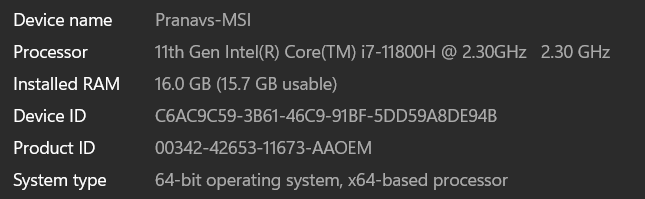
\includegraphics[width=1\textwidth]{screenshot-3.png}\\[1cm]
This PC was used to make this project.

\chapter{Software Used}
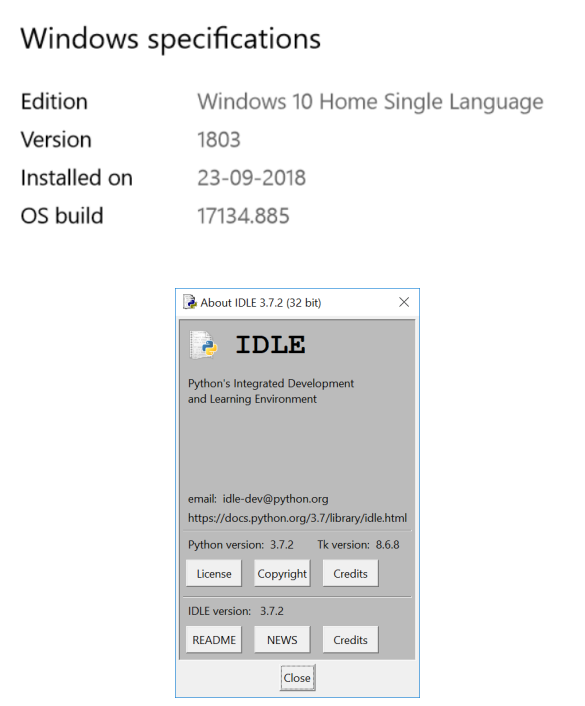
\includegraphics[width=0.8\textwidth]{screenshot-4.png}\\[1cm]
Python 37-32 was used to write the code of this system.

% System Architecture
\chapter{System Architecture}
The main components are organized as follows:

\begin{figure}[h]
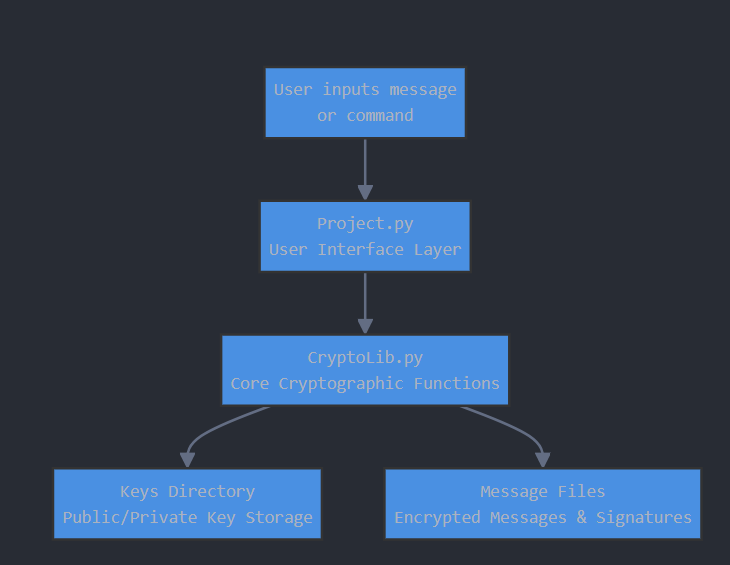
\includegraphics[width=\textwidth]{screenshot-2.png}
\caption{System Architecture Overview}
\end{figure}

The system consists of these key components:
\begin{itemize}
    \item \textbf{Project.py}: Acts as the user interface layer, handling all user interactions and command processing
    \item \textbf{CryptoLib.py}: Contains all core cryptographic functions and utilities for encryption, decryption, and signature operations
    \item \textbf{Keys Directory (/keys)}: Storage for Generated Private and Public Key Pairs
    \item \textbf{Message Files (message.txt)}: Holds the Encrypted Message.
     \item \textbf{Signature File (signature.txt)}: Holds the Sigtuare for a Given Message.
\end{itemize}

\chapter{Screenshots}
\section{All Screenshots}
\subsection{Screenshot 1}
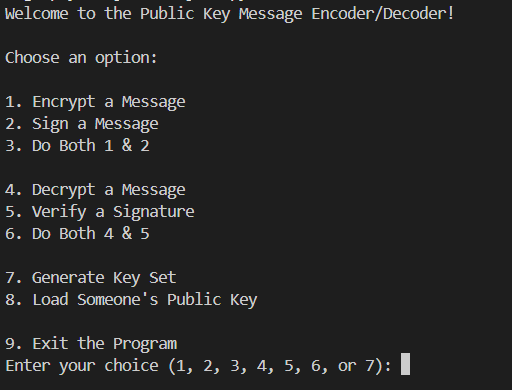
\includegraphics[width=1\textwidth]{screenshot-1.png}
\subsection{Screenshot 2}
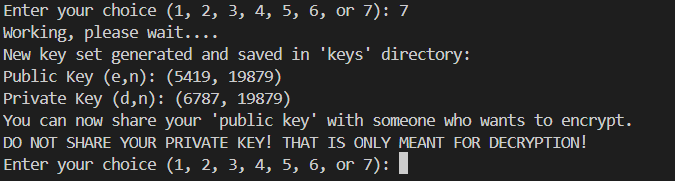
\includegraphics[width=1\textwidth]{screenshot-5.png}
\subsection{Screenshot 3}
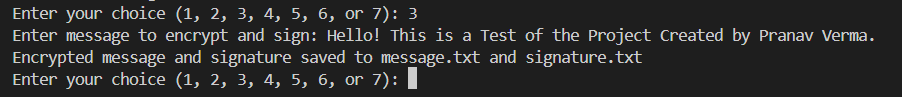
\includegraphics[width=1\textwidth]{screenshot-6.png}
\subsection{Screenshot 4}
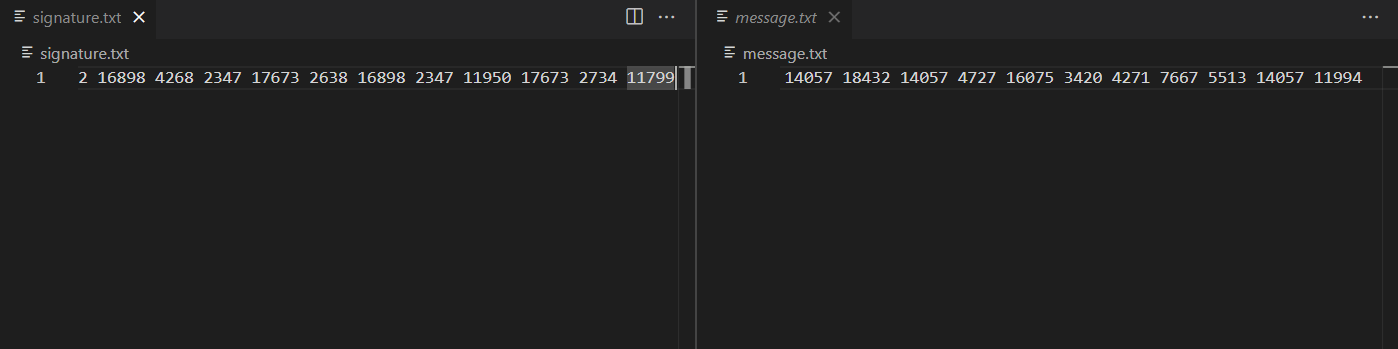
\includegraphics[width=1\textwidth]{screenshot-7.png}
\subsection{Screenshot 5}
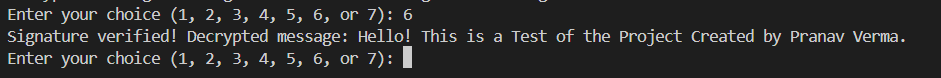
\includegraphics[width=1\textwidth]{screenshot-8.png}


\chapter{Codes}
\section{Project.py}
\begin{lstlisting}[language=Python]
import CryptoLib as lb;
import os;
import sys;

print("Welcome to the Public Key Message Encoder/Decoder!")

print("\nChoose an option:")
print("")
print("1. Encrypt a Message")
print("2. Sign a Message")
print("3. Do Both 1 & 2")
print("")
print("4. Decrypt a Message")
print("5. Verify a Signature")
print("6. Do Both 4 & 5")
print("")
print("7. Generate Key Set")
print("8. Load Someone's Public Key")
print("")
print("9. Exit the Program")


while True:
    choice = input("Enter your choice (1, 2, 3, 4, 5, 6, or 7): ")

    # number 1
    if choice == "1":
        public_key = lb.load_key('keys/public.key')
        message = input("Enter the message to encrypt: ")
        encrypted_message = lb.encryptMessage(message, public_key)
        with open('message.txt', 'w') as f:
            f.write(encrypted_message)
        print("Encrypted message saved to message.txt")

    # number 2
    elif choice == "2":
        private_key = lb.load_key('keys/private.key')
        message = input("Enter the message to sign: ")
        signature = lb.sign_message(message, private_key)
        with open('signature.txt', 'w') as f:
            f.write(signature)
        print("Message signed and saved to signature.txt")
        print("Share both the message and signature.txt with the recipient")

    # number 3
    elif choice == "3":
        recipient_public_key = lb.load_key('keys/public.key')
        sender_private_key = lb.load_key('keys/private.key')
        message = input("Enter message to encrypt and sign: ")
        encrypted_message, signature = lb.encrypt_and_sign(message, recipient_public_key, sender_private_key)
        with open('message.txt', 'w') as f:
            f.write(encrypted_message)
        with open('signature.txt', 'w') as f:
            f.write(signature)
        print("Encrypted message and signature saved to message.txt and signature.txt")

    # number 4
    elif choice == "4":
        private_key = lb.load_key('keys/private.key')
        filename = 'message.txt'
        if not os.path.exists(filename):
            print("File " + filename + " Not Found.")
            exit()
        with open(filename, 'r') as f:
            encrypted_message = f.read().strip()
        decrypted_message = lb.decrypt_message(encrypted_message, private_key)
        print("Decrypted Message:", decrypted_message)
        
    # number 5
    elif choice == "5":
        public_key = lb.load_key('keys/public.key')
        message = input("Enter the original message: ")
        filename = 'signature.txt'
        if not os.path.exists(filename):
            print("File " + filename + " Not Found.")
            exit()
        with open(filename, 'r') as f:
            signature = f.read().strip()
        if lb.verify_signature(message, signature, public_key):
            print("Signature is valid! Message is authentic.")
        else:
            print("Invalid signature! Message may have been tampered with.")

    # number 6
    elif choice == "6":
        sender_public_key = lb.load_key('keys/public.key')
        recipient_private_key = lb.load_key('keys/private.key')
        if (not os.path.exists('signature.txt')):
            print("'signature.txt' Not Found.")
            print("Try Encrypting a Message First.")
            exit()
        if (not os.path.exists('message.txt')):
            print("'message.txt' Not Found.")
            print("Try Encrypting a Message First.")
            exit()
        with open('message.txt', 'r') as f:
            encrypted_message = f.read().strip()
        with open('signature.txt', 'r') as f:
            signature = f.read().strip()
        verified, result = lb.verify_and_decrypt(encrypted_message, signature, sender_public_key, recipient_private_key)
        if verified:
            print("Signature verified! Decrypted message:", result)
        else:
            print("Error:", result)

    # number 7
    elif choice == "7":
        print("Working, please wait....")
        public_key, private_key = lb.generate_keys()
        print("New key set generated and saved in 'keys' directory:")
        print("Public Key (e,n):", public_key)
        print("Private Key (d,n):", private_key)
        print("You can now share your 'public key' with someone who wants to encrypt.")
        print("DO NOT SHARE YOUR PRIVATE KEY! THAT IS ONLY MEANT FOR DECRYPTION!")

    # number 8
    elif choice == "8":
        print("Enter the public key in the format 'e,n'")
        print("Example: 6553,2341")
        key_text = input("Enter public key: ")
        if lb.saveKeyFromText(key_text):
            print("Public key successfully loaded and saved to keys/public.key")
        else:
            print("Error: Invalid key format. Please use the format 'e,n' with numbers only")

    # number 9
    elif choice == "9":
        sys.exit(0)

    else:
        print("Please enter 1, 2, 3, 4, 5, 6, or 7.")
\end{lstlisting}



\section{CryptoLib.py}
\begin{lstlisting}[language=Python]
# Crypto Library w/ all Functions.
# Made by Pranav Verma from XI Raman

import random;
import math;
import os;
import hashlib;

# standard gcd function
def gcd(a, b):
    while b != 0:
        a, b = b, a % b
    return a

def generate_keys():
    primes = []
    for i in range(100, 501):
        is_prime = True
        for j in range(2, int(math.sqrt(i)) + 1):
            if i % j == 0: #check for prime
                is_prime = False
                break
        if is_prime:
            primes.append(i)

    p = random.choice(primes) # random select prime 1
    q = random.choice(primes) # random select prime 2
    while p == q: # the two numbers should not be equal to the other 
        q = random.choice(primes)

    n = p * q # calc. base
    phi = (p - 1) * (q - 1) #eulers totient function

    e = random.randint(2, phi - 1)
    while gcd(e, phi) != 1: # calc gcd
        e = random.randint(2, phi - 1)

    d = pow(e, -1, phi)

    if not os.path.exists('keys'):
        os.makedirs('keys')

    with open('keys/public.key', 'w') as f:
        f.write(f"{e},{n}")

    with open('keys/private.key', 'w') as f:
        f.write(f"{d},{n}")

    return ((e, n), (d, n))

def load_key(filename):
    if not os.path.exists(filename):
        print("Please generate keys first.")
        exit()
    with open(filename, 'r') as f:
        key = f.read().strip().split(',')
        return (int(key[0]), int(key[1]))
    
def saveKeyFromText(key_text):
    try:
        e, n = map(int, key_text.strip().split(','))
        if not os.path.exists('keys'):
            os.makedirs('keys')
            
        with open('keys/public.key', 'w') as f:
            f.write(f"{e},{n}")
        return True
    except:
        return False
    
def encryptMessage(message, public_key):
    e, n = public_key
    encrypted_message = []
    for char in message:
        encrypted_char = (ord(char) ** e) % n
        encrypted_message.append(str(encrypted_char))
    return ' '.join(encrypted_message)

def decrypt_message(encrypted_message, private_key):
    d, n = private_key
    encrypted_chars = encrypted_message.split()
    decrypted_message = ''.join([chr((int(char) ** d) % n) for char in encrypted_chars])
    return decrypted_message

def hash_message(message):
    return hashlib.sha256(message.encode()).hexdigest()

def sign_message(message, private_key):
    d, n = private_key
    message_hash = hash_message(message)
    signature = []
    for char in message_hash:
        # ok how did this actually work
        signed_char = pow(ord(char), d, n)
        signature.append(str(signed_char))
    return ' '.join(signature)

def verify_signature(message, signature, public_key):
    e, n = public_key
    # make the hash from original sig.
    signature_nums = signature.split()
    recovered_hash = ''
    for num in signature_nums:
        char = pow(int(num), e, n)
        recovered_hash += chr(char)
    # compare
    return recovered_hash == hash_message(message)

def encrypt_and_sign(message, recipient_public_key, sender_private_key):
    encrypted_message = encryptMessage(message, recipient_public_key)
    signature = sign_message(encrypted_message, sender_private_key)
    return encrypted_message, signature

def verify_and_decrypt(encrypted_message, signature, sender_public_key, recipient_private_key):
    # verify sig
    if not verify_signature(encrypted_message, signature, sender_public_key):
        return False, "Signature verification failed!"
    # decrpt the message.
    decrypted_message = decrypt_message(encrypted_message, recipient_private_key)
    return True, decrypted_message
\end{lstlisting}

% Bibliography
\chapter{Bibliography}
\begin{enumerate}
    \item Python Documentation - \texttt{hashlib} module
    \item Python Documentation - \texttt{random} module
    \item GeeksForGeeks - \texttt{Eulers Totient Function}
    \item JavatPoint - \texttt{RSA Formula}
\end{enumerate}

\end{document}